% Options for packages loaded elsewhere
\PassOptionsToPackage{unicode}{hyperref}
\PassOptionsToPackage{hyphens}{url}
%
\documentclass[
]{article}
\usepackage{amsmath,amssymb}
\usepackage{iftex}
\ifPDFTeX
  \usepackage[T1]{fontenc}
  \usepackage[utf8]{inputenc}
  \usepackage{textcomp} % provide euro and other symbols
\else % if luatex or xetex
  \usepackage{unicode-math} % this also loads fontspec
  \defaultfontfeatures{Scale=MatchLowercase}
  \defaultfontfeatures[\rmfamily]{Ligatures=TeX,Scale=1}
\fi
\usepackage{lmodern}
\ifPDFTeX\else
  % xetex/luatex font selection
\fi
% Use upquote if available, for straight quotes in verbatim environments
\IfFileExists{upquote.sty}{\usepackage{upquote}}{}
\IfFileExists{microtype.sty}{% use microtype if available
  \usepackage[]{microtype}
  \UseMicrotypeSet[protrusion]{basicmath} % disable protrusion for tt fonts
}{}
\makeatletter
\@ifundefined{KOMAClassName}{% if non-KOMA class
  \IfFileExists{parskip.sty}{%
    \usepackage{parskip}
  }{% else
    \setlength{\parindent}{0pt}
    \setlength{\parskip}{6pt plus 2pt minus 1pt}}
}{% if KOMA class
  \KOMAoptions{parskip=half}}
\makeatother
\usepackage{xcolor}
\usepackage{graphicx}
\makeatletter
\def\maxwidth{\ifdim\Gin@nat@width>\linewidth\linewidth\else\Gin@nat@width\fi}
\def\maxheight{\ifdim\Gin@nat@height>\textheight\textheight\else\Gin@nat@height\fi}
\makeatother
% Scale images if necessary, so that they will not overflow the page
% margins by default, and it is still possible to overwrite the defaults
% using explicit options in \includegraphics[width, height, ...]{}
\setkeys{Gin}{width=\maxwidth,height=\maxheight,keepaspectratio}
% Set default figure placement to htbp
\makeatletter
\def\fps@figure{htbp}
\makeatother
\setlength{\emergencystretch}{3em} % prevent overfull lines
\providecommand{\tightlist}{%
  \setlength{\itemsep}{0pt}\setlength{\parskip}{0pt}}
\setcounter{secnumdepth}{-\maxdimen} % remove section numbering
\ifLuaTeX
  \usepackage{selnolig}  % disable illegal ligatures
\fi
\IfFileExists{bookmark.sty}{\usepackage{bookmark}}{\usepackage{hyperref}}
\IfFileExists{xurl.sty}{\usepackage{xurl}}{} % add URL line breaks if available
\urlstyle{same}
\hypersetup{
  hidelinks,
  pdfcreator={LaTeX via pandoc}}

\author{}
\date{}

\begin{document}

% \hypertarget{a-study-of-deep-learning-based-generative-models-vae-vs-gan}{%
% \section{A Study of Deep Learning Based Generative Models: VAE vs
% GAN}\label{a-study-of-deep-learning-based-generative-models-vae-vs-gan}}
\begin{center}
\section{{A Study of Deep Learning Based Generative Models: VAE vs GAN}}
\end{center}

\begin{center}
\textbf{Shanlong Guo}\\
\textit{University of Florida}\\
\texttt{sh.guo@ufl.edu}
\end{center}

% Shanlong Guo

% University of Florida

% sh.guo@ufl.edu

All code for this report has been uploaded to Github:
\url{https://github.com/TerryGSL/MLProject.git}

\begin{center}
\hypertarget{abstract}{%
\subsection{Abstract}\label{abstract}}
\end{center}


In this project report, I mainly learn the basic principles of two major
generative models GAN and VAE, and use them to generate some new images,
the main dataset used is mnist, from the comparison of the generated
results I found that the images generated by VAE are more blurred, while
the images generated by GAN are realistic, but its potential space may
not have good structure.

Since the images generated using GAN are more noisy, I also studied a
variant model of GAN, DCGAN, which optimizes the network structure based
on GAN and makes the network easier to train. I first used it to
generate some new mnist handwritten digital images and found that the
generated images are of higher quality and more stable for training.
Then I used a crawler to crawl some anime images in anime websites and
crop them, then I used DCGAN to generate new anime avatars on top of
that dataset, and the final avatars I got were very good.

Finally, I found a paper which describes a new hybrid generation model:
CVAE-GAN, which combines the advantages of CVAE and GAN, using CVAE to
encode the input and GAN to generate the image, and can use the prior
probability distribution of CVAE to control the generated image
properties, and also can improve the generated image by the adversarial
loss function of GAN to improve the So I tried to reproduce the model of
this paper to generate mnist handwritten digits, and I ended up with
good results, and I was also able to generate the specified different
styles of digits, and also observe how one digit is slowly converted
into another one.

\hypertarget{1-introduction}{%
\subsection{1 Introduction}\label{1-introduction}}

With the rapid development of deep learning, generative models have
attracted more and more attention in recent years. Among various
generative models, generative adversarial networks (GAN) and variational
autoencoders (VAE) are two widely used and studied models.

GANs can generate high-quality images similar to real images, but they
suffer from training instability and pattern collapse problems. On the
other hand, VAE can generate diverse images, but the image quality is
lower. Therefore, researchers have been exploring how to combine the
advantages of GAN and VAE to overcome their limitations.

In this project, we investigated the basic principles of GAN and VAE and
used them to generate new images in the MNIST dataset. We found that
although GAN generates more realistic images, its latent space may not
have a well-organized structure. vae generates more diverse images, but
the image quality is lower.

To improve the stability and image quality of GAN, we also explored the
DCGAN model, which optimizes the network structure of GAN and shows
better training stability and image quality. We applied DCGAN to a new
anime face dataset and obtained high quality and diverse anime face
images.

Finally, we investigate a new hybrid model, called CVAE-GAN, which
combines the advantages of CVAE and GAN. The model uses CVAE to encode
the input and GAN to generate the images, and the generated image
attributes can be controlled by the prior probability distribution of
CVAE. We implemented the CVAE-GAN model on the MNIST dataset and
achieved good results, including the ability to generate different
styles of figures and observe a gradual shift from one figure to
another.

In summary, this project outlines the basic principles of GAN and VAE
and their limitations, explores the DCGAN model for better image quality
and stability, and investigates a new hybrid model, CVAE-GAN, which has
the potential to generate high-quality images with controllable
attributes.

\hypertarget{2-related-work}{%
\subsection{2 Related Work}\label{2-related-work}}

In recent years, there has been a growing interest in applying deep
learning techniques to the field of image generation, and Generative
Adversarial Network (GAN) and Variational Autoencoder (VAE) are two of
the most widely used models.

GAN was proposed by Goodfellow et al. (2014), which showed impressive
results because it can generate high quality images similar to real
images. However, the training process of GAN is unstable, so it may lead
to some crashes or low-quality image generation. To address these
issues, several modifications to GAN architectures have been proposed,
such as Wasserstein GAN (Arjovsky et al., 2017) and Spectral
Normalization GAN (Miyato et al., 2018).

In contrast, VAE was introduced by Kingma and Welling (2013), it aim to
learn a probabilistic distribution of the input data, and it allow for
the generation of new samples from the learned distribution. While VAE
are able to generate diverse samples, they often produce lower quality
images compared to GAN due to the weaker reconstruction loss. Various
modifications have been proposed to improve the quality of VAE-generated
images, such as β-VAE (Higgins et al., 2017) and Adversarial
Autoencoders (Makhzani et al., 2016). VAE have also been used in various
image generation tasks, such as 3D shape generation (Wu et al., 2016)
and face generation (Larsen et al., 2015).

To leverage the strengths of both GANs and VAEs, hybrid models have been
proposed, such as Adversarial Autoencoder (Makhzani et al., 2016) and
Adversarial Variational Bayes (Mescheder et al., 2017). These models aim
to learn a low-dimensional latent representation of the input data using
the encoder component of a VAE, which is then used to generate new
samples using the decoder component of a GAN. Another hybrid model,
CVAE-GAN (Zhao et al., 2017), uses the prior distribution learned by the
VAE to control the image attributes during the GAN\textquotesingle s
image generation process.

In summary, GAN and VAE have been extensively studied and have made
significant progress in image generation tasks. Various modifications
and hybrid models have been proposed to overcome the limitations of each
individual model, and have shown impressive results in generating
high-quality and diverse images.

\hypertarget{3-deep-generative-models-review}{%
\subsection{3 Deep Generative Models
Review}\label{3-deep-generative-models-review}}

\hypertarget{31-gan}{%
\subsubsection{3.1 GAN}\label{31-gan}}

A discriminator and a generator work together in the GAN, an alternate
method for producing data based on a given prior distribution.\\
The generator creates images from random noise, which is frequently
referred to as an eigenvector or code and is typically derived from a
uniform distribution (homogeneous distribution) or a Gaussian
distribution, while the discriminator is used to distinguish "true" and
"false" images.\\
The generator\textquotesingle s job is to create a fakeable image that
even the discriminator will have trouble identifying. In other words,
the discriminator and the generator are at odds with one another. The
generator does its best to produce more realistic images so that the
discriminator would classify them as true, while the discriminator works
very hard to discriminate between true and false images.

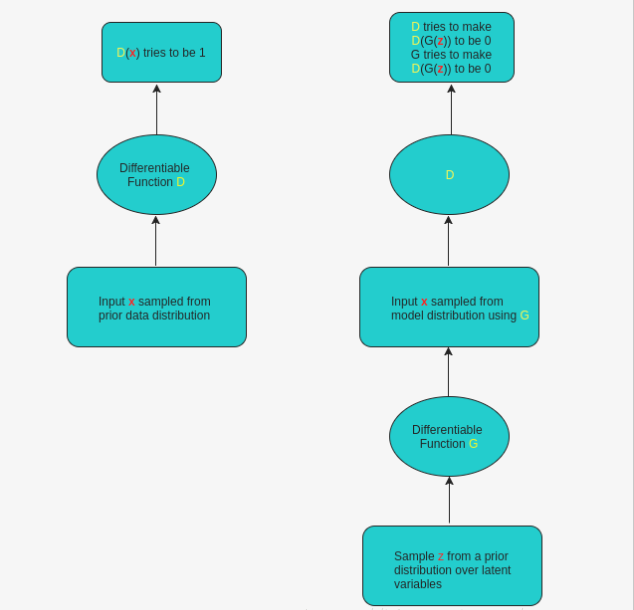
\includegraphics{image-20230419235444754.png}

Let\textquotesingle s say we have the networks G (generator) and D
(discriminator), respectively. The generator network G aims to produce
realistic visuals during training in an effort to trick the
discriminator network D. D\textquotesingle s objective is to attempt to
distinguish between the fake images produced by G and the real ones. G
and D create a dynamic "game process" in this manner.

This principle can be expressed in the following equation:

Suppose we have a training set \(S={x(1),... ,x(m)}\). Moreover, given
any probability density function \(pz(z)\) (of course, the simpler the
corresponding probability distribution is, the better, while keeping the
model complexity), we can use the random variable \(Z∼pz(z)\) to sample
\(m\) noisy samples \({z(1),...,z(m)}\). ,z(m)\}\$. From this, we can
obtain the likelihood function:
$$
\begin{aligned}
L&(x^{(1)}, \ldots, x^{(m)}, z^{(1)}, \ldots, z^{(m)} \mid \theta_{g}, \theta_{d}) \\
&= \prod_{i=1}^{m} D(x^{(i)})^{I\{x^{(i)} \in \text{Data}\}}(1-D(x^{(i)}))^{I\{x^{(i)} \notin \text{Data}\}} \\
&\qquad\qquad\times \prod_{j=1}^{m} D(G(x^{(j)}))^{I\{G(x^{(j)}) \in \text{Data}\}}(1-D(G(x^{(j)})))^{I\{G(x^{(j)}) \notin \text{Data}\}} \\
&= \prod_{i=1}^{m} D(x^{(i)}) \prod_{j=1}^{m} (1-D(G(x^{(j)})))
\end{aligned}
$$
Further, the log-likelihood is obtained as:
$$
\begin{aligned}
\log L &= \log \left(\prod_{i=1}^{m} D\left(x^{(i)}\right) \prod_{j=1}^{m}\left(1-D\left(G\left(x^{(j)}\right)\right)\right)\right) \\
&= \sum_{i=1}^{m} \log D\left(x^{(i)}\right)+\sum_{j=1}^{m} \log \left(1-D\left(G\left(z^{(j)}\right)\right)\right)
\end{aligned}
$$
By the law of large numbers, when \(m → ∞\), we approximate the expected
loss by the empirical loss and obtain:
$$
\log L \approx \mathrm{E}_{x \sim p_{\text {data }}(x)}[\log D(x)]+\mathrm{E}_{z \sim p_z(z)}[\log (1-D(x))] \mid
$$
On the one hand, we want to optimize the learnable parameters of the
discriminator to maximize the log-likelihood function, and on the other
hand, we want to optimize them to reduce the log-likelihood function.
Formalizing this leads to the following optimization goal:
$$
\min _G \max _D V(D, G)=\mathbb{E}_{\boldsymbol{x} \sim p_{\text {data }}(\boldsymbol{x})}[\log D(\boldsymbol{x})]+\mathbb{E}_{\boldsymbol{z} \sim p_{\boldsymbol{z}}(\boldsymbol{z})}[\log (1-D(G(\boldsymbol{z})))]
$$
\begin{itemize}
\item
  There are just two terms in the entire equation. In the following, "x"
  stands for the actual image, "z" for the noise input to the G network,
  and "G(z)" for the image produced by the G network.
\item
  Since x is the real image, the closer this value is to 1 for D, the
  more likely the D network is to identify that \textbf{the real picture
  is real}. And D(G(z)) is the likelihood that the \textbf{D network
  will decide whether or not the G-generated picture is accurate. }
\item
  The goal of G: as stated above, D(G(z)) is the likelihood** that the D
  network will discern whether the image produced by G is real or not.
  In other words, since V(D, G) will be tiny, G wants D(G(z)) to be as
  large as feasible. Thus, we can see that min\_G is the
  equation\textquotesingle s top notation.
\item
  The goal of D: the larger D(x) and the smaller D(G(x)) should be, the
  more capable D is. The size of V(D,G) will increase at this point. In
  order to determine the maximum value for D, the equation is (max\_D).
\end{itemize}

Here, D and G are trained using the stochastic gradient descent
approach. This is how the algorithm works:

 \begin{figure}[htbp]
    \centering 
    \includegraphics{1.jpg} 
\end{figure}

The first phase is training D. D is adding the gradient (ascending) in
an effort to make V(G, D) as big as it can be. The gradient is
subtracted (descending) in the second step of our training process for G
such that V(G, D) is as minimal as possible. Alternating training
methods are used throughout.

\hypertarget{32-dcgan}{%
\subsubsection{3.2 DCGAN}\label{32-dcgan}}

CNN and GAN are combined to create DCGAN. Convolutional networks are
incorporated into the generative model to do unsupervised training, and
the powerful feature extraction capabilities of convolutional networks
are used to enhance the generative network\textquotesingle s learning
capabilities.

The basic idea behind DCGAN is the same as that of GAN, with the
exception that two convolutional neural networks (CNNs) take the place
of G and D in GAN, and DCGAN modifies the design of convolutional neural
networks to enhance sample quality and convergence speed:

\begin{itemize}
\item
  There are no longer any pooling layers. The G network uses a
  transposed convolutional layer for upsampling, and the D network
  substitutes stride convolution for pooling.
\item
  Both D and G use batch normalization.
\item
  To convert the network into a completely convolutional network, remove
  the FC layer.
\item
  Tanh is employed in the bottom layer while ReLU is used as the
  activation function in the G network.
\item
  The activation function in the D network is LeakyReLU.
\end{itemize}

Schematic representation of the G network in DCGAN:

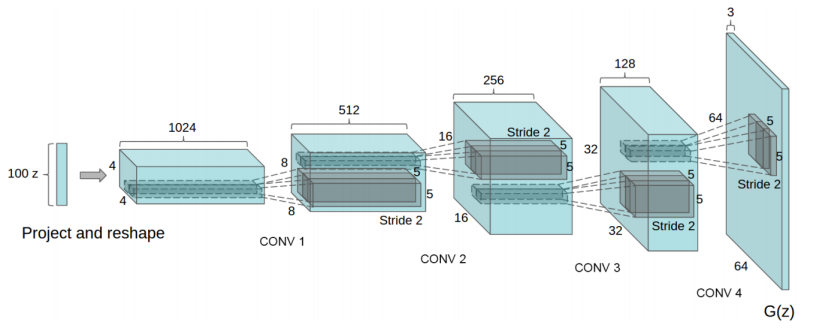
\includegraphics{DCGAN_generator.png}

As can be seen, the input of the generator is a 100-dimensional noise,
and the middle will pass through 4 convolution layers, with each
convolution layer halving the number of channels and doubling the length
and width to produce a 64\emph{64}3 size image output. It should be
noted that many papers citing DCGAN make the mistaken assumption that
the four convolutional layers are \textbf{Wide Convolution} when, in
fact, they are \textbf{Fractionally Strided Convolution}. The difference
between the two is illustrated in the figure below:

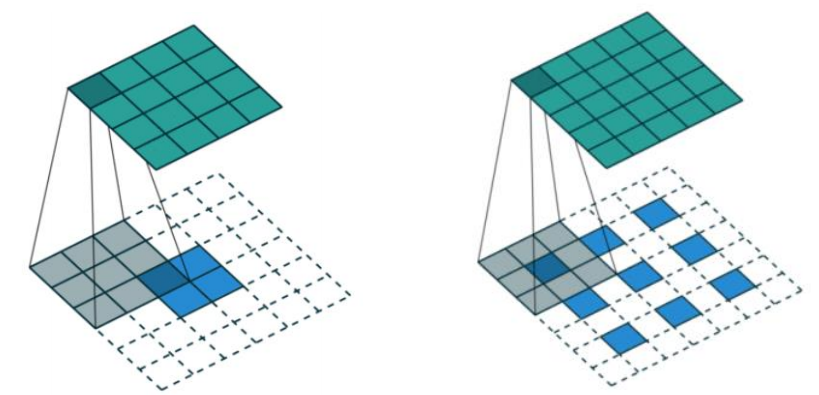
\includegraphics{卷积层比较.png}

In contrast to micro-step amplitude convolution, which divides the input
matrix and adds zeros around each individual pixel point, broad
convolution adds zeros around the whole input matrix.

The above two \textbf{convolutional} operations that map from
low-dimensional features to high-dimensional features are called
\textbf{transpose convolution}, also known as deconvolution.

\hypertarget{33-vae}{%
\subsubsection{3.3 VAE}\label{33-vae}}

A priori data distributions can be modeled using the variational
self-encoder. It is made up of an encoder and a decoder. A latent vector
is a low-level representation of the data that is created by the encoder
by mapping high-level properties of the data distribution. The
data\textquotesingle s low-level representations are ingested by the
decoder, which then produces its high-level counterparts.

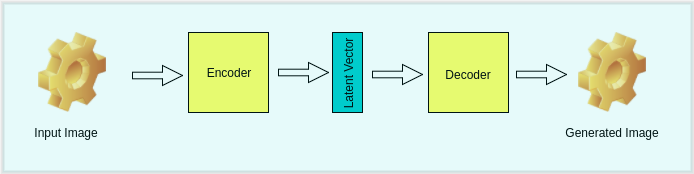
\includegraphics{06859image (12).png}

% \hypertarget{331-variational-lower-bound}{%
% \paragraph{3.3.1 Variational Lower
% bound}\label{331-variational-lower-bound}}
{\bfseries \small 3.3.1 Variational Lower bound} \\
Additionally, the posterior probability is typically maximized to optimize the created model. That is, using the Bayesian formulation:
$$
p(z \mid X)=\frac{p(X \mid z) p(z)}{\int_z p(X \mid z) p(z) \mathrm{d} z}
$$
We want to replace the posterior probability \(p(z|X)\) with the new
function \(q(z)\), then the two probability distributions need to be as
similar as possible, and here the KL scatter is still chosen to measure
the closeness of the two. According to the KL formula then we have:
$$
\begin{aligned}
\mathrm{KL}(q(z) \| p(z \mid X)) & =\int q(z) \log \frac{q(z)}{p(z \mid X)} \mathrm{d} z \\
& =\int q(z)[\log q(z)-\log p(z \mid X)] \mathrm{d} z
\end{aligned}
$$
Transformation according to the Bayesian formula yields:
$$
\begin{aligned}
& =\int q(z)\left[\log q(z)-\log \frac{p(X \mid z) p(X)}{p(z)}\right] \mathrm{d} z \\
& =\int q(z)[\log q(z)-\log p(X \mid z)-\log p(z)+\log p(X)] \mathrm{d} z
\end{aligned}
$$
Since the objective of the integration is z, the items that are not
related to z are then taken out of the integration notation to obtain:
$$
=\int q(z)[\log q(z)-\log p(X \mid z)-\log p(z)] \mathrm{d} z+\log p(X)
$$
Swapping the equation left and right yields the following equation:
$$
\log p(X)-\mathrm{KL}(q(z) \| p(z \mid X))=\int q(z) \log p(X \mid z) \mathrm{d} z-\mathrm{KL}(q(z) \| p(z))
$$
The goal of our training is to want
KL(q(z)\textbar\textbar p(z\textbar X)) to be as small as possible,
which is equivalent to making the right side of the equal sign as large
as possible. The first term on the right side of the equal sign is
actually based on the log-likelihood expectation of the probability of
\(q(z)\), and the second term is again a negative KL scatter, so we can
assume that in order to find a good \(q(z)\) that makes it as similar as
possible to \(p(z|X)\) and achieve the final optimization goal, the
optimization objective will become:
$$
\begin{aligned}
&\max \int q(z) \log p(X \mid z) \mathrm{d} z\\
&\min \operatorname{KL}(q(z)|| p(z))
\end{aligned}
$$
{\bfseries \small 3.3.2 Reparameterization Trick} \\
% \hypertarget{332-reparameterization-trick}{%
% \paragraph{3.3.2 Reparameterization
% Trick}\label{332-reparameterization-trick}}
The variational function \(q(z)\), which, to approximate the posterior
probability, actually represents the distribution of z given some X,
would be \(q(z|X)\) if its probability form were written in its
entirety. We need to find a way to abstract it out of X. This
conditional probability can be split into two parts, one is an observed
variable \(gϕ(X)\), which represents the deterministic part of the
conditional probability and its value is similar to the expectation of a
random variable; the other part is the random variable \(ε\), which is
responsible for the random part. If \(z(i)=gϕ(X+ε(i))\), then
\(q(z(i))=p(ε(i))\), so the above formula on the derivation of the
variance can be turned into the following one:
$$
\log p(X)-\operatorname{KL}(q(z) \| p(z \mid X))=\int p(\varepsilon) \log p\left(X \mid g_\phi(X, \varepsilon)\right) \mathrm{d} z-\operatorname{KL}(q(z \mid X, \varepsilon) \| p(z))
$$
This assumption ϵ obeys a multidimensional and independent Gaussian
distribution in each dimension. Also, the prior and posterior of z are
assumed to be a multidimensional and independent Gaussian distribution
in each dimension. The final form of the two optimization objectives is
shown below.

% \hypertarget{333-encoder-and-decoder-formula}{%
% \paragraph{3.3.3 Encoder and Decoder
% formula}\label{333-encoder-and-decoder-formula}}
{\bfseries \small 3.3.3 Encoder and Decoder formula} \\
Getting the second term \(KL(q(z)||p(z)))\) on the right side of
Equation as small as possible is our second optimization goal. The prior
of \(z\) is currently assumed to be a multidimensional and independent
Gaussian distribution in each dimension, and a stronger assumption can
be made here that the mean of each dimension of this Gaussian
distribution is zero and the covariance is the unit matrix. From this
point, the previously mentioned KL scatter formula begins with:
$$
\operatorname{KL}(p 1 \| p 2)=\frac{1}{2}\left[\log \frac{\operatorname{det}\left(\Sigma_2\right)}{\operatorname{det}\left(\Sigma_1\right)}-\mathrm{d}+\operatorname{tr}\left(\Sigma_2^{-1} \Sigma_1\right)+\left(\mu_2-\mu_1\right)^{\mathrm{T}} \Sigma_2^{-1}\left(\mu_2-\mu_1\right)\right]
$$
Simplified as:
$$
\mathrm{KL}(p 1 \| N(0, I))=\frac{1}{2}\left[-\log \left[\operatorname{det}\left(\Sigma_1\right)\right]-\mathrm{d}+\operatorname{tr}\left(\Sigma_1\right)+\mu_1^{\mathrm{T}} \mu_1\right]
$$
A vector \(σ1\) to represent the major diagonal of the covariance matrix
is all that is required in the calculation, eliminating the necessity to
describe the covariance as the shape of a matrix. The formula will then
be further reduced as follows:
$$
\mathrm{KL}\left(p 1\left(\mu_1, \sigma_1\right) \| N(0, I)\right)=\frac{1}{2}\left[-\sum_i \log \left[\left(\sigma_{1 i}\right)\right]-\mathrm{d}+\sum_i\left(\sigma_{1 i}\right)+\mu_1^{\mathrm{T}} \mu_1\right]
$$
This paradigm is known as the encoder model since the function \(gϕ()\)
carries out the transformation from the observed data to the implied
data.

The next optimization objective, which is to maximize the likelihood
expectation of the first term on the left side of Equation. This part is
relatively simple. Since the previous Encoder model has already
calculated a batch of observed variables \(X\) corresponding to the
implied variables \(z\), another deep model can be built here, modeled
according to the likelihood, with the input being the implied variables
\(z\) and the output being the observed variables \(X\). If the output
image is similar to the previously generated image, then the likelihood
is considered to be maximized. This model is called Decoder.

\hypertarget{34-cvae-gan}{%
\subsubsection{3.4 CVAE-GAN}\label{34-cvae-gan}}

The CVAE-GAN model combines the advantages of CVAE and GAN with better
control, stability and diversity, and is a very effective generative
model. Where C stands for the ability to generate images for a specified
classification using the classification as input. It generates images
quite well on each classification as shown in the following figure.

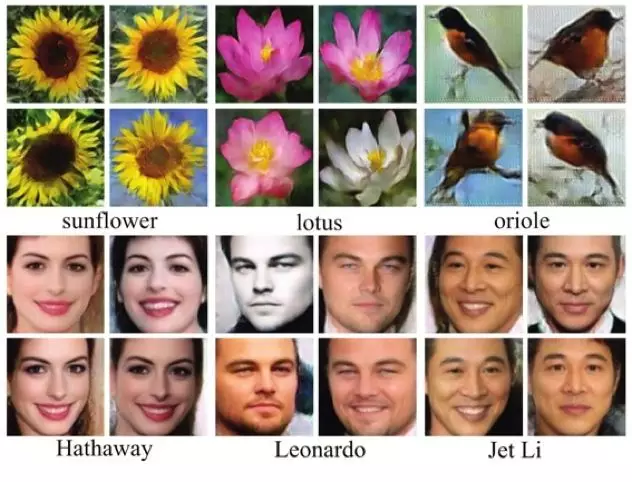
\includegraphics{1528778328059.png}

CVAE-GAN is mainly composed of the following 4 neural networks:

\begin{itemize}
\item
  E: Encoder (Encoder), input image x, output encoding z.
\item
  G: Generator. Input encoding z, output image x.
\item
  C: Classifier. Input image x, output category c.
\item
  D: Discriminator. Input image x, determine its truthfulness.
\end{itemize}

The architecture of CVAE-GAN is shown in the following figure:

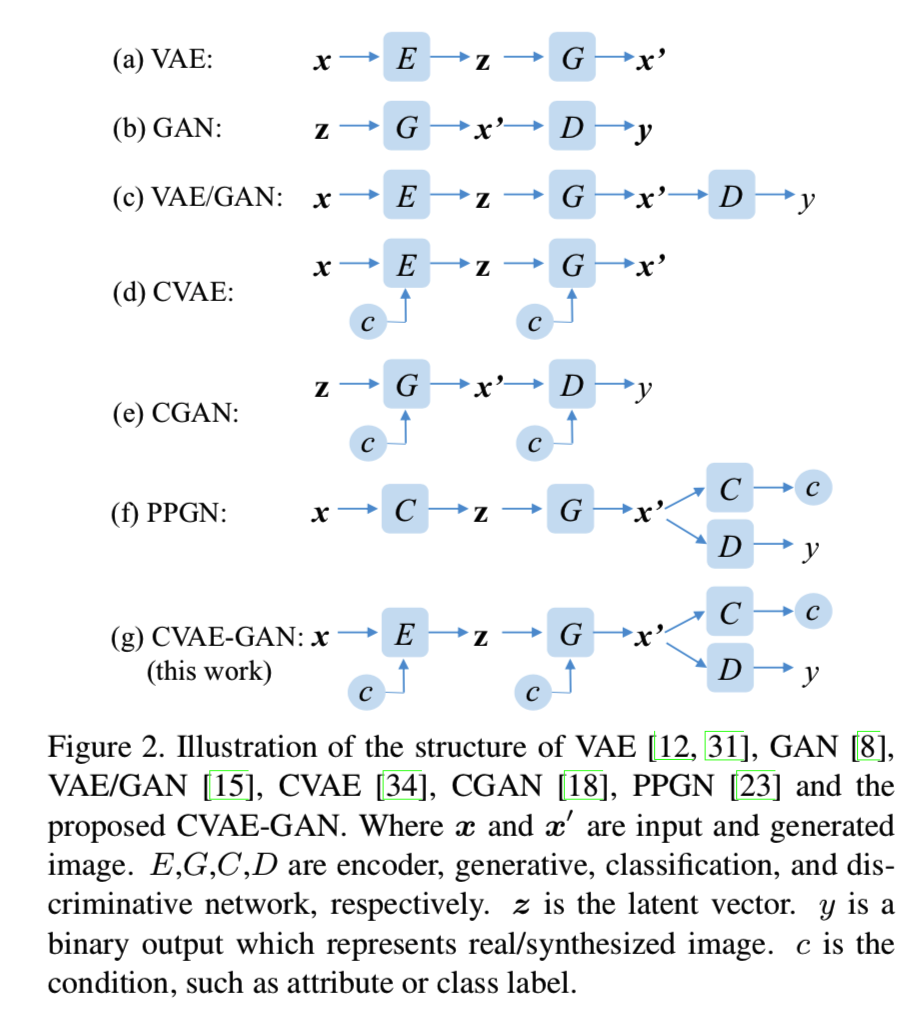
\includegraphics{1446032-20190909111131054-1070453947.png}

The G of VAE is better than the G of GAN, so the structure of VAE is in
front. Then, since VAE\textquotesingle s criterion for judging
x\textquotesingle{} and x similarity is not good enough, we have to add
D again to judge it. Finally, we need to ensure that the generated image
belongs to the c-category, so C is also added.

where the Loss of G has three main parts:

\begin{itemize}
\item
  For z generated from x, G should be able to restore
  x\textquotesingle{} close to x (pixel-wise close)
\item
  The image generated by G should be identifiable by D as belonging to
  the real image
\item
  the image generated by G should be identifiable by C as belonging to
  category c
\end{itemize}

The resulting z can be fairly well carved out of the image.

The detailed architecture of CVAE-GAN is shown in Fig:

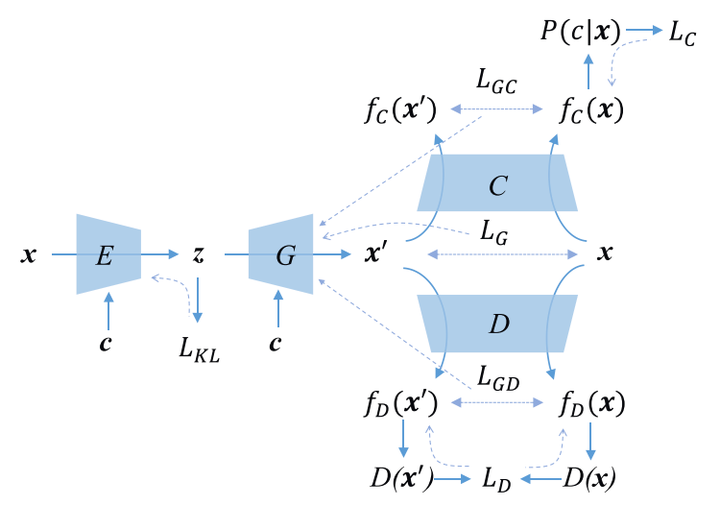
\includegraphics{v2-a07b6a20ff4de63aa937f269bcec92ea_720w.png}

The training algorithm of CVAE-GAN is shown in the figure, where each
item is intuitive. Note that there is also an important trick used in
it, which is to expect x\textquotesingle{} and x to have similar
features in the middle layers of the network for D and C. This helps
stabilize the network: x\textquotesingle{} and x\textquotesingle{} have
similar features in the middle layers. This helps to stabilize the
network:

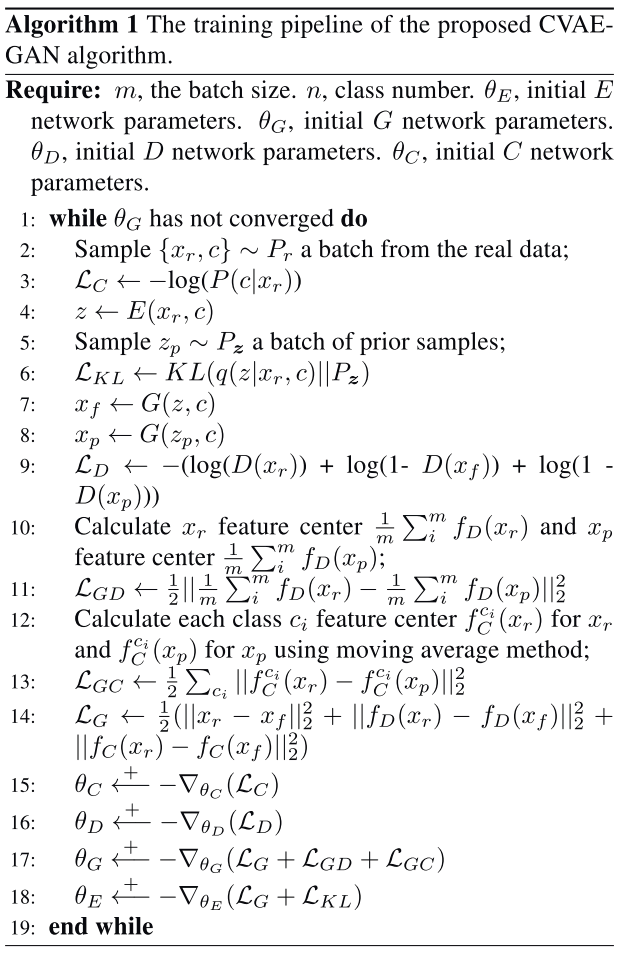
\includegraphics{v2-8127b9b611186785a9d4ca3046752cee_720w.png}

By using the four major networks E+G+C+D, CVAE-GAN achieves a fairly
satisfactory generative model.

\hypertarget{4-results}{%
\subsection{4 Results}\label{4-results}}

In total, we tested GAN, DCGAN, VAE, CVAE-GAN on handwritten digital
datasets and also extraordinarily used DCGAN on top of our own crawled
anime dataset and got good results. All the experimental codes are
implemented using Pytorch, and the initial size of our mnist dataset
images is \(28\times28\), and the initial size of anime images is
\(256\times256\).

Here are some specific experimental results to show and some of our
hyperparameter choices.

\hypertarget{41-gan}{%
\subsubsection{4.1 GAN}\label{41-gan}}

\textbf{Hyper-parameters :}

latent\_size = 64

hidden\_size = 256

image\_size = 784

num\_epochs = 200

batch\_size = 100

lr = 0.0002

\textbf{Optimizer : adam optimizer}

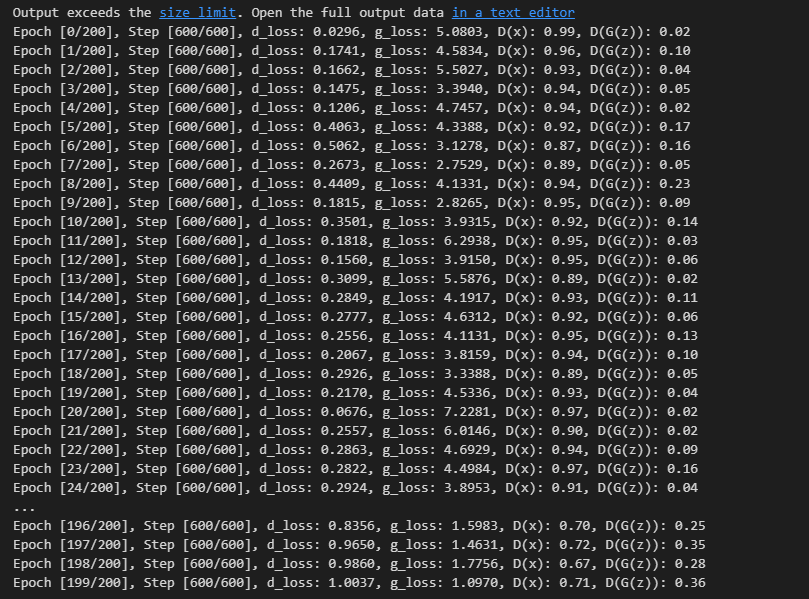
\includegraphics{image-20230420023436403.png}

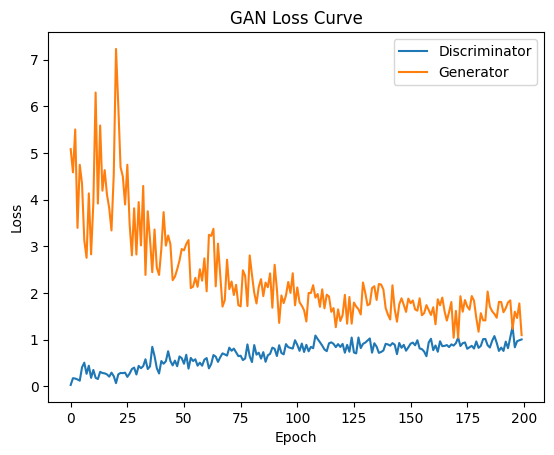
\includegraphics{image-20230420023443142.png}

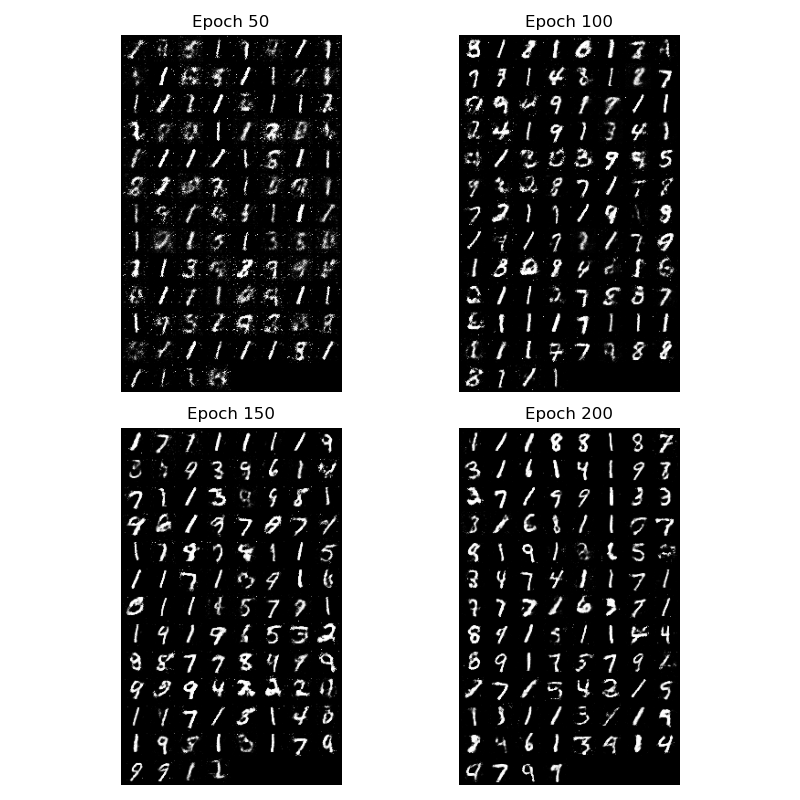
\includegraphics{merged_img_gan.png}

\hypertarget{42-dcgan}{%
\subsubsection{4.2 DCGAN}\label{42-dcgan}}

\textbf{Dataset: mnist}

\textbf{Hyper-parameters :}

batch\_size = 128

num\_epoch = 100

z\_dimension = 100

lr = 0.0003

\textbf{Optimizer : adam optimizer}

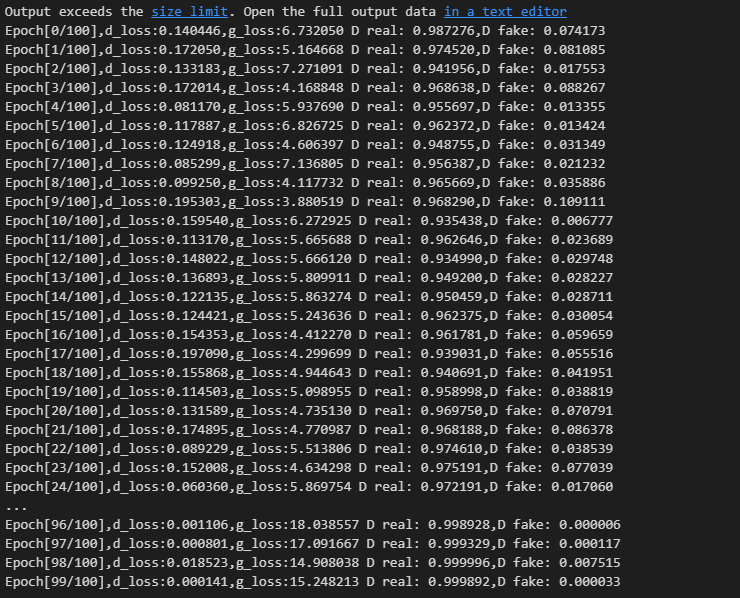
\includegraphics{image-20230420023639790.png}

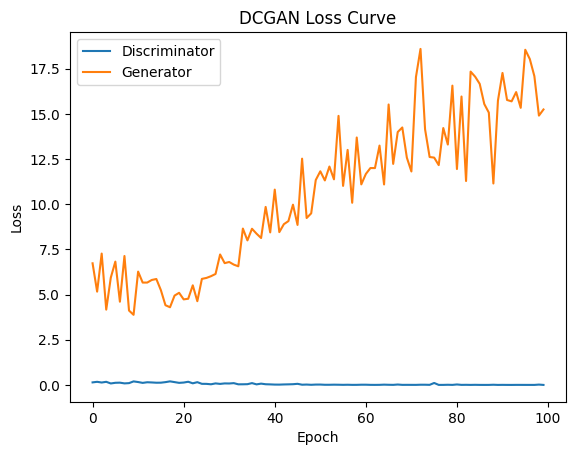
\includegraphics{image-20230420023647382.png}

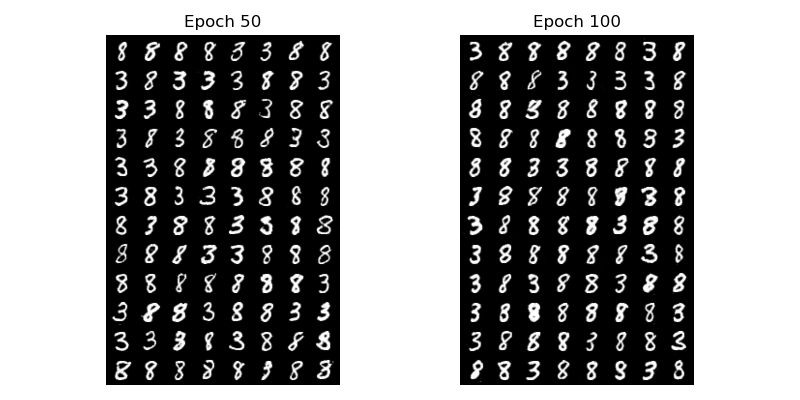
\includegraphics{merged_img_dcgan.png}

\textbf{Dataset: anime}

Random Seed: 999

workers = 2

batch\_size = 128

image\_size = 64

since images are RGB they have 3 channels: nc = 3

generator input size: nz = 100

generator\textquotesingle s feature maps: ngf = 64

discriminator\textquotesingle s feature maps: ndf = 64

num\_epochs = 50

lr = 0.0002

beta1 = 0.5

\textbf{Optimizer : adam optimizer}

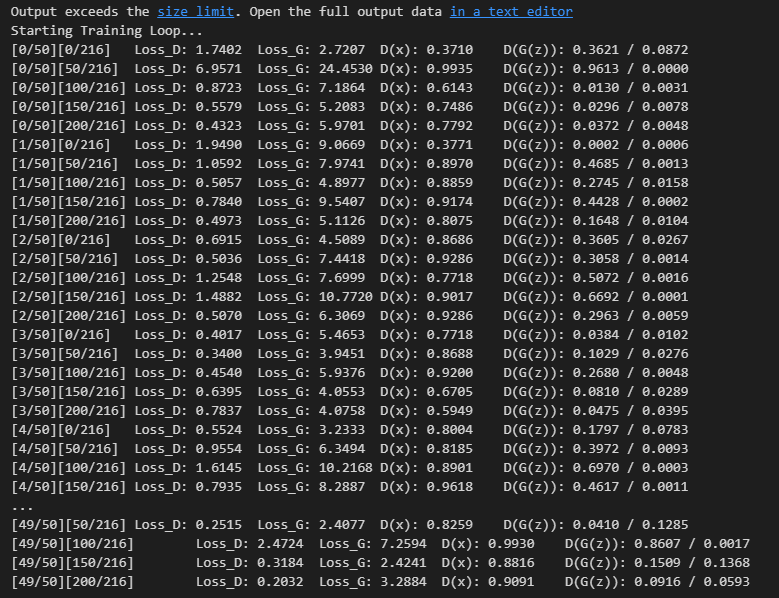
\includegraphics{image-20230420024107792.png}

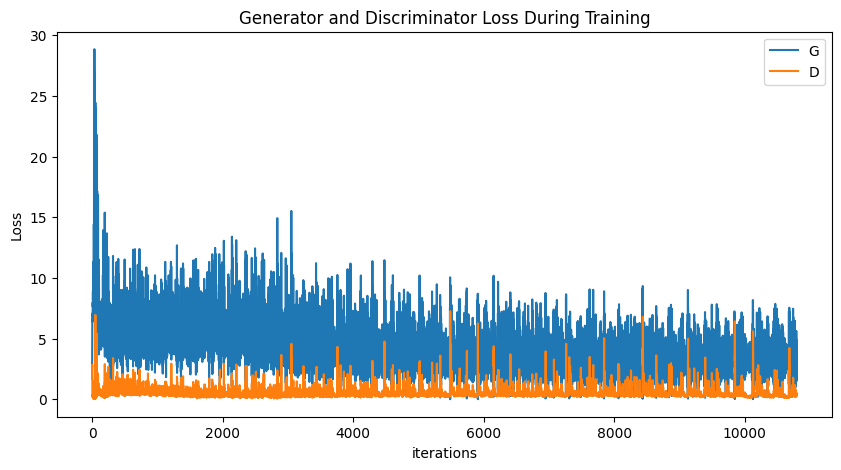
\includegraphics{image-20230420024113949.png}

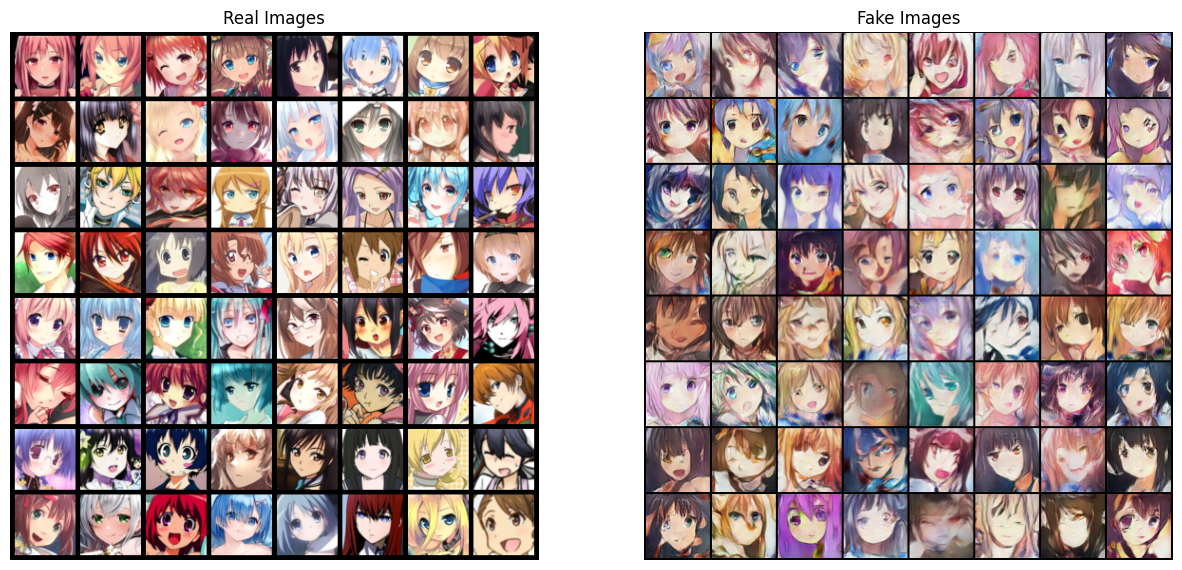
\includegraphics{image-20230420024120310.png}

\hypertarget{43-vae}{%
\subsubsection{4.3 VAE}\label{43-vae}}

latent\_dim = 2

input\_dim = 28 * 28

inter\_dim = 256

epochs = 200

batch\_size = 128

lr = 0.0001

\textbf{Optimizer : adam optimizer}

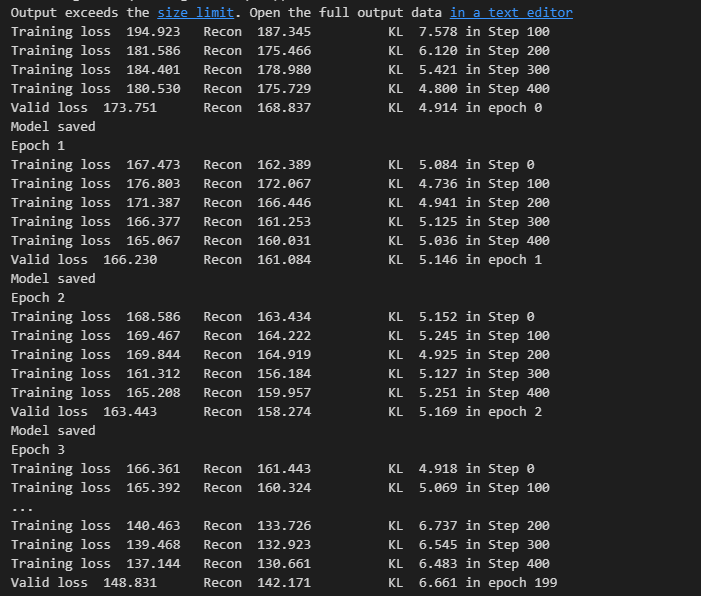
\includegraphics{image-20230420024836582.png}

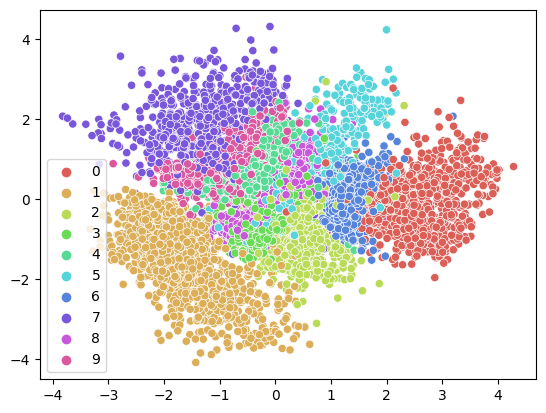
\includegraphics{image-20230420024842829.png}

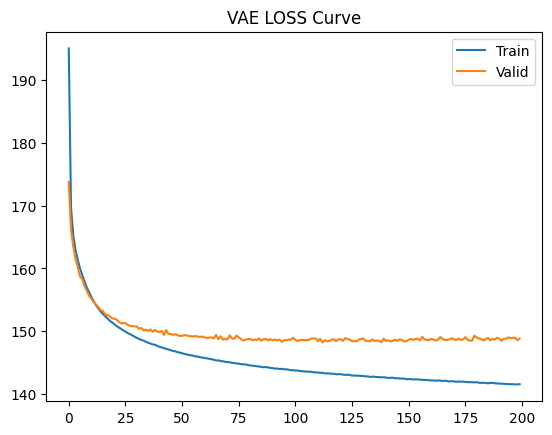
\includegraphics{image-20230420024847966.png}

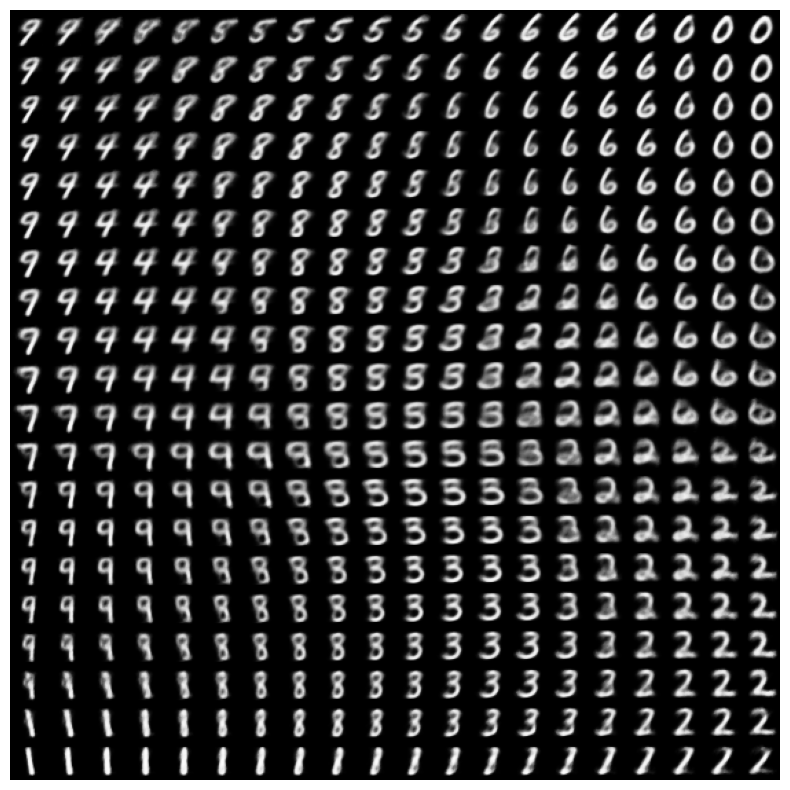
\includegraphics{image-20230420024856105.png}

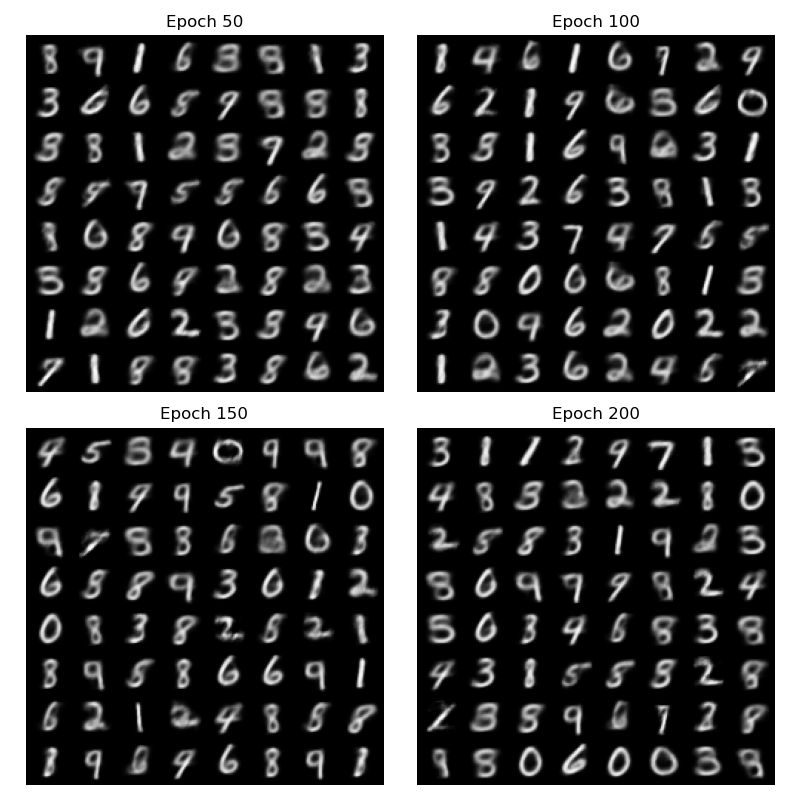
\includegraphics{merged_img.png}

\hypertarget{44-cvae-gan}{%
\subsubsection{4.4 CVAE-GAN}\label{44-cvae-gan}}

batchSize = 128

imageSize = 28

nz = 100

nepoch = 200

Random Seed: 88

lr = 0.0001

\textbf{Optimizer : adam optimizer}

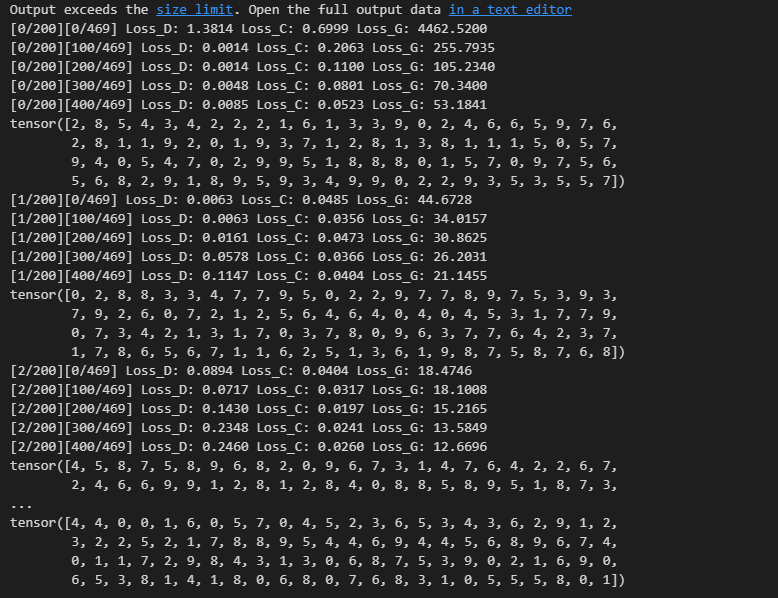
\includegraphics{image-20230420025106706.png}

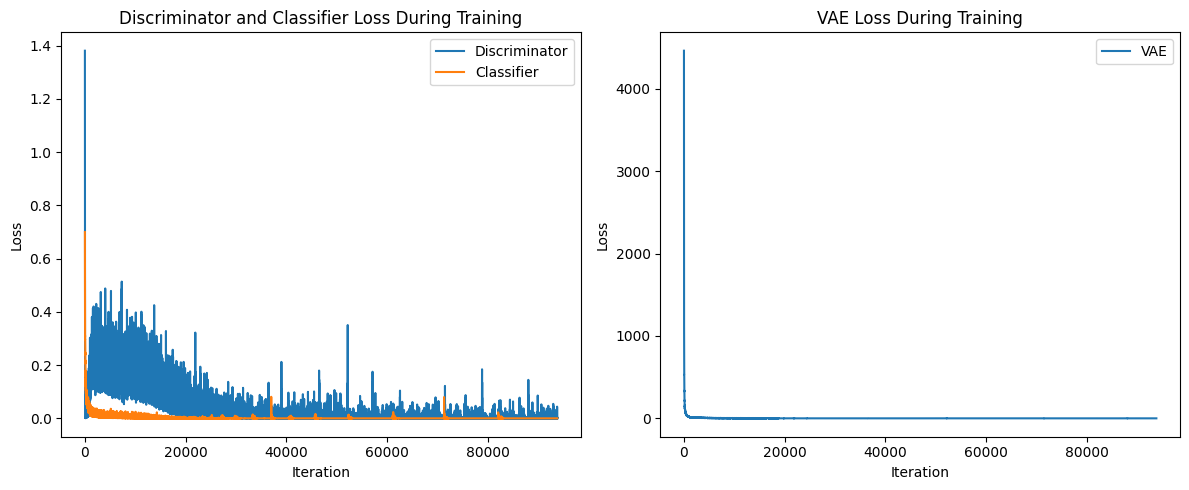
\includegraphics{image-20230420025113062.png}

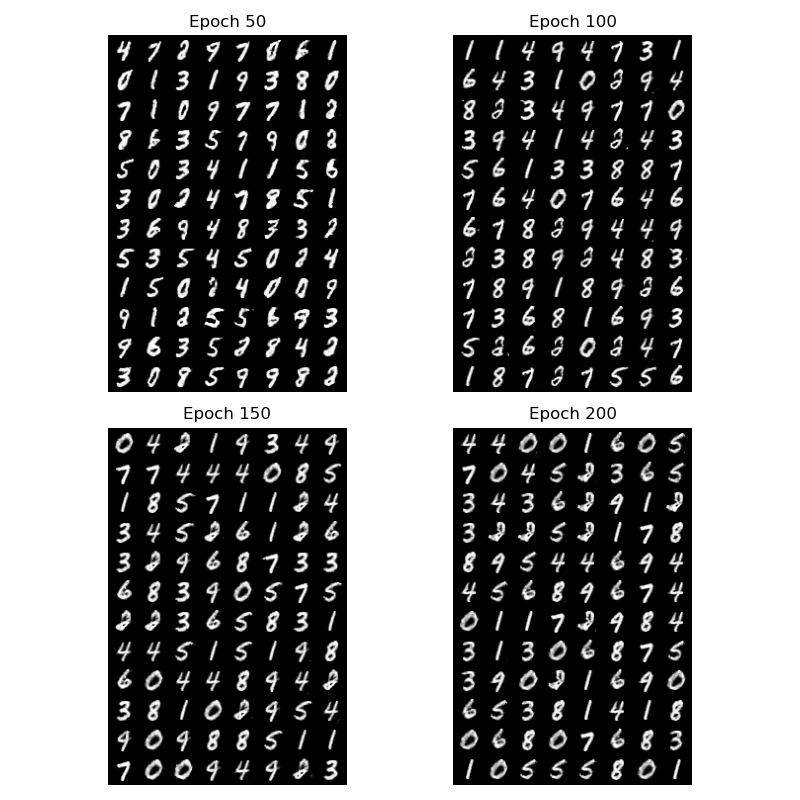
\includegraphics{merged_img_cvaegan.png}

\textbf{Specify the generated image:}

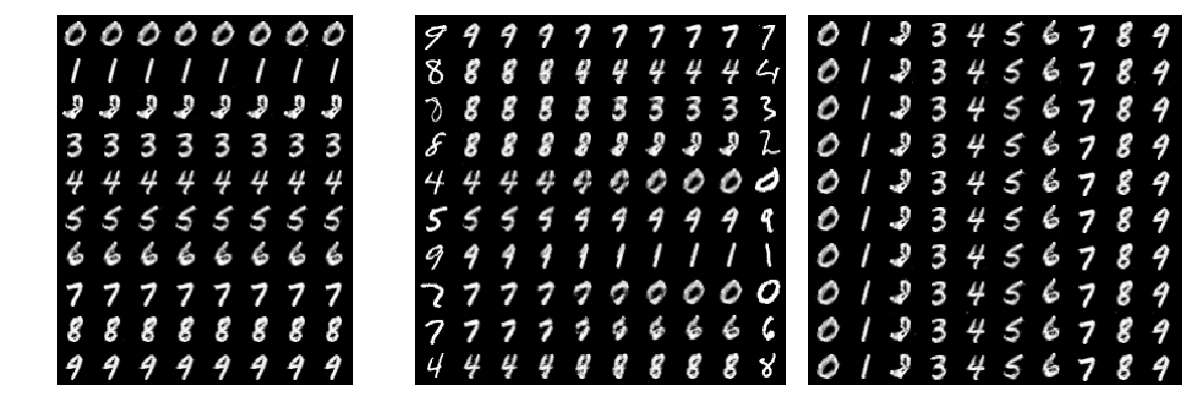
\includegraphics{merged_img-1681974949975-45.png}

\hypertarget{5-conclusion}{%
\subsection{5 Conclusion}\label{5-conclusion}}

We evaluate and compare the performance of GAN, DCGAN, VAE, and CVAE-GAN
on the MNIST dataset as well as on our own collection of anime face
datasets. The results show that although GANs produce high-quality
images that are visually similar to real images, they suffer from
instability and pattern collapse problems during training. On the other
hand, VAEs produce diverse images but with lower image quality. the
DCGAN model shows better image quality and stability during training.
the CVAE-GAN model combines the advantages of both models to produce
high-quality images with controllable properties.

From the experimental results, we found that the DCGAN model outperforms
the traditional GAN model in terms of image quality and training
stability. The generated anime face images show high diversity and
quality, which demonstrates the effectiveness of the DCGAN architecture
in learning complex image features.

In addition, we observe that the VAE model is able to generate diverse
images but with lower image quality compared to the GAN and DCGAN
models. This is because the VAE model is optimized for reconstruction
loss rather than for image generation. Nevertheless, the VAE model
provides a useful tool to explore the latent space and generate new
images from the learned distributions.

The CVAE-GAN model shows impressive results in generating high-quality
images with controllable properties. By using the prior distribution
learned by CVAE, we are able to control the image properties during
image generation by GAN. This allows us to generate different styles of
figures on the MNIST dataset and create smooth transitions between two
different figures.

To achieve these results, we faced several challenges in the training
process. A major issue is the instability of the GAN training process,
which causes the model to produce low-quality images or collapse into a
single pattern. To address this issue, we tried different modifications
to the GAN architecture, such as DCGAN, and found that these
modifications improved the stability of the training process.

Another challenge is to choose the appropriate hyperparameters for each
model, such as learning rate and batch size. We performed a grid search
to find the best values of these hyperparameters, which allowed us to
achieve the best results for each model.

In addition, our anime face dataset is relatively small and contains a
wide range of styles, which makes it difficult for us to achieve good
image quality and diversity. We addressed this issue by pre-processing
the images and using data enhancement techniques to increase the size of
the dataset.

In summary, this project provides insights into the strengths and
limitations of GAN, VAE and their hybrid models. We successfully applied
these models to generate high-quality images on the MNIST dataset and
our own anime face dataset. our experimental results demonstrate the
potential of deep learning models in generating high-quality and diverse
images. We also identified and overcame several challenges, including
training instability and hyperparameter selection. Our results
demonstrate the potential of these models in generating high quality and
diverse images with controlled attributes.

\begin{center}
\hypertarget{references}{%
\subsection{References}\label{references}}
\end{center}


{[}1{]} Goodfellow, Ian, et al. "Generative adversarial networks."
\emph{Communications of the ACM} 63.11 (2020): 139-144.

{[}2{]} Arjovsky, Martin, Soumith Chintala, and Léon Bottou.
"Wasserstein generative adversarial networks." \emph{International
conference on machine learning}. PMLR, 2017.

{[}3{]} Miyato, Takeru, et al. "Spectral normalization for generative
adversarial networks." \emph{arXiv preprint arXiv:1802.05957} (2018).

{[}4{]} Kingma, Diederik P., and Max Welling. "Auto-encoding variational
bayes." \emph{arXiv preprint arXiv:1312.6114} (2013).

{[}5{]} Higgins, Irina, et al. "beta-vae: Learning basic visual concepts
with a constrained variational framework." \emph{International
conference on learning representations}. 2017.

{[}6{]} Larsen, Anders Boesen Lindbo, et al. "Autoencoding beyond pixels
using a learned similarity metric." \emph{International conference on
machine learning}. PMLR, 2016.

{[}7{]} Wu, Jiajun, et al. "Learning a probabilistic latent space of
object shapes via 3d generative-adversarial modeling." \emph{Advances in
neural information processing systems} 29 (2016).

{[}8{]} Makhzani, Alireza, et al. "Adversarial autoencoders."
\emph{arXiv preprint arXiv:1511.05644} (2015).

{[}9{]} Mescheder, Lars, Sebastian Nowozin, and Andreas Geiger.
"Adversarial variational bayes: Unifying variational autoencoders and
generative adversarial networks." \emph{International conference on
machine learning}. PMLR, 2017.

{[}10{]} Bao, Jianmin, et al. "CVAE-GAN: fine-grained image generation
through asymmetric training." \emph{Proceedings of the IEEE
international conference on computer vision}. 2017.

\end{document}